% ============================================================================
% Context-Aware Extension to GraDeT-HTR
% Comprehensive Technical Report
% ============================================================================
\documentclass[11pt, a4paper]{report}

% --- Core ---
\usepackage[utf8]{inputenc}
\usepackage[T1]{fontenc}
\usepackage{lmodern}
\usepackage[english]{babel}
\usepackage{geometry}
\geometry{margin=2.5cm}

% --- Mathematics ---
\usepackage{amsmath, amssymb, amsthm}
\usepackage{mathtools}

% --- Graphics and Figures ---
\usepackage{tikz}
\usetikzlibrary{
  arrows.meta,
  calc,
  decorations.pathreplacing,
  fit,
  matrix,
  positioning,
  shapes.geometric,
  backgrounds,
  patterns
}
\usepackage{pgfplots}
\pgfplotsset{compat=1.18}
\usepackage{graphicx}
\usepackage{subcaption}

% --- Code Listings ---
\usepackage{listings}
\usepackage{xcolor}
\usepackage[most]{tcolorbox}

% --- Tables ---
\usepackage{booktabs}
\usepackage{multirow}
\usepackage{tabularx}
\usepackage{colortbl}
\usepackage{longtable}

% --- Typography ---
\usepackage{microtype}
\usepackage{enumitem}
\usepackage[colorlinks=true, linkcolor=blue!70!black, citecolor=blue!70!black, urlcolor=blue!70!black]{hyperref}
\usepackage[capitalise,noabbrev]{cleveref}
\usepackage{fancyhdr}

% --- Algorithms ---
\usepackage{algorithm}
\usepackage{algpseudocode}

% --- Page Style ---
\pagestyle{fancy}
\fancyhf{}
\fancyhead[L]{\leftmark}
\fancyhead[R]{\thepage}
\renewcommand{\headrulewidth}{0.4pt}

% ============================================================================
% Custom Environments
% ============================================================================

% Python listing style
\lstdefinestyle{pythonstyle}{
  language=Python,
  basicstyle=\ttfamily\scriptsize,
  keywordstyle=\color{blue!80!black}\bfseries,
  stringstyle=\color{red!60!black},
  commentstyle=\color{green!50!black}\itshape,
  numbers=left,
  numberstyle=\tiny\color{gray},
  numbersep=5pt,
  breaklines=true,
  showstringspaces=false,
  tabsize=4,
  frame=none,
  xleftmargin=1em,
  morekeywords={self, None, True, False, torch, Optional, int, float, bool, str},
}

% Original code box (red-tinted)
\newtcblisting{originalcode}[1][]{%
  colback=red!3!white,
  colframe=red!50!black,
  title={\small\textbf{Original} \texttt{#1}},
  fonttitle=\small\ttfamily,
  listing only,
  listing options={style=pythonstyle, numbers=left},
  breakable,
  enhanced,
  boxrule=0.6pt,
  left=2pt, right=2pt, top=0pt, bottom=0pt,
  before skip=6pt, after skip=6pt,
}

% New code box (green-tinted)
\newtcblisting{newcode}[1][]{%
  colback=green!3!white,
  colframe=green!50!black,
  title={\small\textbf{New (Extension)} \texttt{#1}},
  fonttitle=\small\ttfamily,
  listing only,
  listing options={style=pythonstyle, numbers=left},
  breakable,
  enhanced,
  boxrule=0.6pt,
  left=2pt, right=2pt, top=0pt, bottom=0pt,
  before skip=6pt, after skip=6pt,
}

% Highlight box for key equations
\newtcolorbox{keyequation}[1][]{%
  colback=blue!5!white,
  colframe=blue!60!black,
  title={#1},
  fonttitle=\bfseries,
  enhanced,
  boxrule=0.6pt,
}

% Generic code listing
\newtcblisting{codebox}[1][]{%
  colback=gray!3!white,
  colframe=gray!50!black,
  title={\small\texttt{#1}},
  fonttitle=\small\ttfamily,
  listing only,
  listing options={style=pythonstyle, numbers=left},
  breakable,
  enhanced,
  boxrule=0.6pt,
  left=2pt, right=2pt, top=0pt, bottom=0pt,
}

% ============================================================================
% Title
% ============================================================================
\title{%
  \vspace{-1cm}
  \textbf{Context-Aware Extension to GraDeT-HTR}\\[0.5em]
  \Large Dual-Path Training with Margin Loss for\\Bengali Handwritten Text Recognition\\[1em]
  \large Technical Report --- Extension Work Documentation
}
\author{%
  Md.\ Mahmudul Hasan \and Ahmed Nesar Tahsin Choudhury \and Mahmudul Hasan \and Md.\ Mosaddek Khan\\[0.5em]
  \normalsize Computer Science and Engineering, University of Dhaka
}
\date{\today}

% ============================================================================
\begin{document}
% ============================================================================

\maketitle
\thispagestyle{empty}

% --- Abstract ---
\begin{abstract}
This report documents the context-aware extension to GraDeT-HTR, a Bengali Handwritten Text Recognition system published at EMNLP 2025 System Demonstrations. The base system employs a decoder-only transformer (DTrOCR) with grapheme-based tokenization, achieving state-of-the-art performance on Bengali HTR benchmarks (CER 6.19\%, WER 14.20\% on BN-HTRd). We extend the architecture with a \emph{dual-path training} paradigm that leverages the previously-recognized word as linguistic context. A novel loss function combines standard cross-entropy for both contextual and isolation paths with a margin penalty term $\lambda \cdot \max(0, \mathcal{L}_{\mathrm{ctx}} - \mathcal{L}_{\mathrm{iso}})$ that penalizes samples where context \emph{hurts} recognition accuracy. The extension modifies 6 source files, introduces a new \texttt{ContextAwareDataset} class, implements fixed-length context padding for batch-compatible training, and includes a comprehensive diagnostic test suite of 18 test cases. We detail the theoretical foundation, architecture design with embedding reordering, the complete data flow from context to output, and provide side-by-side code comparisons marking all new additions.
\end{abstract}

\tableofcontents
\newpage

% ============================================================================
\chapter{Introduction and Motivation}
\label{ch:introduction}
% ============================================================================

\section{The Base System --- GraDeT-HTR (EMNLP 2025)}
\label{sec:base-system}

GraDeT-HTR~\cite{gradet2025} is a \textbf{Gra}pheme-aware \textbf{De}coder-only \textbf{T}ransformer for Bengali \textbf{H}andwritten \textbf{T}ext \textbf{R}ecognition, published at the 2025 Conference on Empirical Methods in Natural Language Processing (EMNLP), System Demonstrations track. The system establishes a three-stage pipeline:

\begin{enumerate}[leftmargin=2em]
  \item \textbf{Line Segmentation}: BN-DRISHTI (YOLOv5) detects text lines from full-page images, applying Hough line and affine transformations for deskewing.
  \item \textbf{Word Segmentation}: A second YOLOv5 model segments each line into individual word images.
  \item \textbf{Text Recognition}: DTrOCR, a decoder-only transformer, converts each $32 \times 128$ word image into Bengali grapheme sequences using autoregressive decoding.
\end{enumerate}

\noindent The recognition model (DTrOCR) is the core architectural contribution:
\begin{itemize}[leftmargin=2em]
  \item \textbf{Visual Encoding}: ViT patch embeddings divide each $32 \times 128$ image into $4 \times 8$ non-overlapping patches, producing $N = (32/4) \times (128/8) = 128$ patch tokens, each linearly projected to 768 dimensions.
  \item \textbf{Text Decoding}: 12 GPT-2 transformer blocks with causal (autoregressive) self-attention process the concatenated sequence $[\text{IMAGE}_1, \ldots, \text{IMAGE}_{128}, \text{BOS}, t_1, \ldots, t_T, \text{EOS}]$.
  \item \textbf{Tokenization}: A custom Bengali grapheme tokenizer (BnGraphemizer) with 1296 graphemes (vocabulary size 1420 including special tokens) replaces standard BPE, providing one-to-one mapping between visually coherent units and model tokens.
  \item \textbf{Language Model Head}: A linear projection $\mathbb{R}^{768} \to \mathbb{R}^{1420}$ maps hidden states to vocabulary logits.
\end{itemize}

\noindent The model achieves state-of-the-art results with only 87M parameters, trained from scratch without a pretrained Bengali language model:

\begin{table}[h]
\centering
\caption{GraDeT-HTR base system performance (EMNLP 2025).}
\label{tab:base-results}
\begin{tabular}{lcccc}
\toprule
\multirow{2}{*}{\textbf{Model}} & \multicolumn{2}{c}{\textbf{BN-HTRd}} & \multicolumn{2}{c}{\textbf{Bongabdo}} \\
\cmidrule(lr){2-3} \cmidrule(lr){4-5}
& CER (\%) & WER (\%) & CER (\%) & WER (\%) \\
\midrule
Word\_BnG\_Random (Ours) & \textbf{6.19} & \textbf{14.20} & \textbf{8.68} & \textbf{23.56} \\
Word\_BPE\_Pretrained & 7.57 & 16.30 & 11.61 & 26.99 \\
Word\_BPE\_Random & 6.68 & 15.05 & 10.09 & 25.39 \\
Gemini 2.5 Flash & 19.39 & 32.49 & 37.42 & 56.39 \\
\bottomrule
\end{tabular}
\end{table}

\section{Motivation for Context-Aware Recognition}
\label{sec:motivation}

The base DTrOCR system processes each word image \emph{in complete isolation}---the model has no knowledge of what preceded or follows the current word. In handwritten documents, however, adjacent words carry strong linguistic context:

\begin{itemize}[leftmargin=2em]
  \item \textbf{Linguistic constraints}: Knowing that the previous word is a preposition constrains the space of plausible next words to nouns, pronouns, or adjectives.
  \item \textbf{Disambiguation}: Many Bengali grapheme sequences are visually similar. Context from the previous word can disambiguate between candidates that look identical in isolation.
  \item \textbf{Error recovery}: If a grapheme is partially obscured or poorly written, context provides a prior that can compensate for missing visual information.
\end{itemize}

This observation motivates the central question of this extension: \emph{Can we inject linguistic context from the previously-recognized word into the decoder-only transformer to improve recognition accuracy?}

\section{Contributions Summary}
\label{sec:contributions}

This extension introduces:
\begin{enumerate}[leftmargin=2em]
  \item A \textbf{dual-path training paradigm} where each word image is processed twice per training step---once with the previous word as context and once in isolation---forcing the model to learn both context-aware and context-free recognition.
  \item A \textbf{novel loss function} with a margin penalty term $\lambda \cdot \max(0, \mathcal{L}_{\mathrm{ctx}} - \mathcal{L}_{\mathrm{iso}})$ that explicitly penalizes samples where context \emph{degrades} performance.
  \item An \textbf{embedding reordering mechanism} that inserts context tokens before image patches in the transformer's input sequence, enabling causal attention from image patches to context tokens.
  \item A \textbf{comprehensive diagnostic test suite} (18 test cases, 1020+ lines) validating dimension correctness, gradient flow, loss formula accuracy, and backward compatibility.
\end{enumerate}

% ============================================================================
\chapter{Theoretical Foundation}
\label{ch:theory}
% ============================================================================

\section{Problem Formulation}
\label{sec:problem}

\paragraph{Standard HTR.} Given a word image $\mathbf{x} \in \mathbb{R}^{3 \times 32 \times 128}$, predict a grapheme sequence $\mathbf{y} = (y_1, y_2, \ldots, y_T)$ where each $y_t \in \mathcal{V}$ (vocabulary of 1420 tokens). The model factorizes the joint probability autoregressively:
\begin{equation}
  P(\mathbf{y} \mid \mathbf{x}) = \prod_{t=1}^{T} P(y_t \mid y_{<t}, \mathbf{x})
\end{equation}

\paragraph{Context-Aware HTR.} Given word image $\mathbf{x}$ \emph{and} the previous word's text $\mathbf{c} = (c_1, c_2, \ldots, c_K)$, the contextual probability is:
\begin{equation}
  P(\mathbf{y} \mid \mathbf{x}, \mathbf{c}) = \prod_{t=1}^{T} P(y_t \mid y_{<t}, \mathbf{x}, \mathbf{c})
\end{equation}

We define two per-sample negative log-likelihoods:
\begin{align}
  \mathcal{L}_{\mathrm{iso}} &= -\frac{1}{T-1} \sum_{t=1}^{T-1} \log P(y_t \mid y_{<t}, \mathbf{x}) \quad \text{(isolation path)} \\
  \mathcal{L}_{\mathrm{ctx}} &= -\frac{1}{T-1} \sum_{t=1}^{T-1} \log P(y_t \mid y_{<t}, \mathbf{x}, \mathbf{c}) \quad \text{(contextual path)}
\end{align}

\section{The Dual-Path Loss Function}
\label{sec:loss-function}

\begin{keyequation}[Dual-Path Loss with Margin Penalty]
For each sample $i$ in a batch of size $B$:
\begin{equation}
\boxed{
  \mathcal{L} = \frac{1}{B} \sum_{i=1}^{B} \left[ \underbrace{\mathcal{L}_{\mathrm{ctx}}^{(i)}}_{\text{Term 1}} + \underbrace{\mathcal{L}_{\mathrm{iso}}^{(i)}}_{\text{Term 2}} + \underbrace{\lambda \cdot \max\!\Big(0,\; \mathcal{L}_{\mathrm{ctx}}^{(i)} - \mathcal{L}_{\mathrm{iso}}^{(i)}\Big)}_{\text{Term 3: Margin Penalty}} \right]
}
\label{eq:loss}
\end{equation}
\end{keyequation}

\paragraph{Term 1: Contextual Cross-Entropy ($\mathcal{L}_{\mathrm{ctx}}$).} Trains the model to recognize Bengali graphemes given both the word image \emph{and} the previous word's text as context. This is the standard negative log-likelihood computed from the forward pass with context tokens prepended.

\paragraph{Term 2: Isolation Cross-Entropy ($\mathcal{L}_{\mathrm{iso}}$).} Trains the model to recognize the same word using only the image, without any context. This ensures the model maintains strong image-only recognition capability and does not become dependent on context.

\paragraph{Term 3: Margin Penalty ($\lambda \cdot \max(0, \mathcal{L}_{\mathrm{ctx}} - \mathcal{L}_{\mathrm{iso}})$).} A hinge-like regularization term that activates \emph{only when context hurts}---i.e., when the contextual path produces a higher loss (worse recognition) than the isolation path. When active, it provides an additional gradient signal pushing the model to ensure that context \emph{always helps}.

\paragraph{Probability-to-loss-space conversion.} The original formula is expressed in probability space as $\max(0, P_i - P_c)$, where $P_i = \exp(-\mathcal{L}_{\mathrm{ctx}})$ is the contextual probability and $P_c = \exp(-\mathcal{L}_{\mathrm{iso}})$ is the isolation probability. This fires when $P_i < P_c$, which is equivalent to $\mathcal{L}_{\mathrm{ctx}} > \mathcal{L}_{\mathrm{iso}}$ in loss space. We use the loss-space approximation $\max(0, \mathcal{L}_{\mathrm{ctx}} - \mathcal{L}_{\mathrm{iso}})$ which has the same activation condition and cleaner gradients.

\begin{figure}[t]
\centering
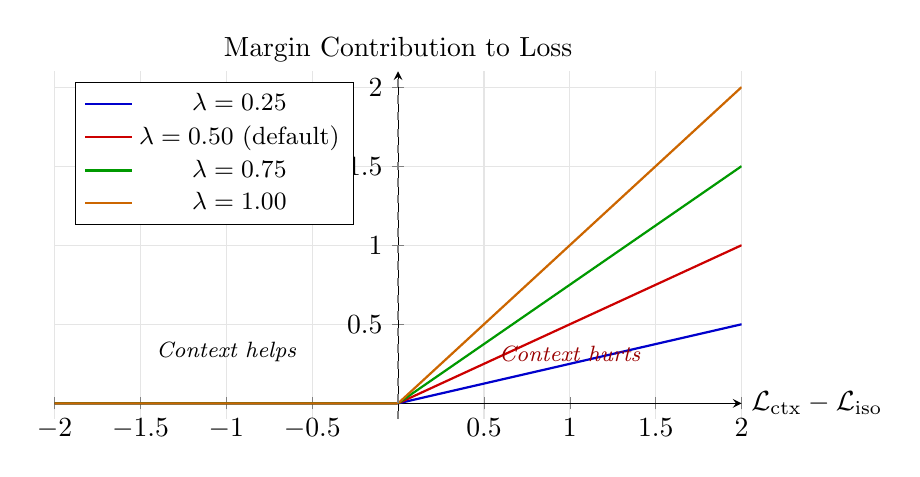
\begin{tikzpicture}
\begin{axis}[
  width=0.85\textwidth,
  height=6cm,
  xlabel={$\mathcal{L}_{\mathrm{ctx}} - \mathcal{L}_{\mathrm{iso}}$},
  ylabel={Margin Contribution to Loss},
  xmin=-2, xmax=2,
  ymin=-0.1, ymax=2.1,
  grid=major,
  grid style={gray!20},
  legend pos=north west,
  legend style={font=\small},
  axis lines=middle,
  every axis x label/.style={at={(ticklabel* cs:1.0)}, anchor=west},
  every axis y label/.style={at={(ticklabel* cs:1.0)}, anchor=south},
]
\addplot[blue!80!black, thick, domain=-2:2, samples=200]
  {max(0, 0.25*x)};
\addlegendentry{$\lambda = 0.25$}
\addplot[red!80!black, thick, domain=-2:2, samples=200]
  {max(0, 0.5*x)};
\addlegendentry{$\lambda = 0.50$ (default)}
\addplot[green!60!black, thick, domain=-2:2, samples=200]
  {max(0, 0.75*x)};
\addlegendentry{$\lambda = 0.75$}
\addplot[orange!80!black, thick, domain=-2:2, samples=200]
  {max(0, 1.0*x)};
\addlegendentry{$\lambda = 1.00$}
\addplot[gray, dashed, thick] coordinates {(0,-0.1) (0,2.1)};

\node[anchor=south, font=\footnotesize\itshape] at (axis cs:-1.0,0.2) {Context helps};
\node[anchor=south, font=\footnotesize\itshape, red!60!black] at (axis cs:1.0,0.2) {Context hurts};
\end{axis}
\end{tikzpicture}
\caption{Margin penalty contribution as a function of the loss difference $\mathcal{L}_{\mathrm{ctx}} - \mathcal{L}_{\mathrm{iso}}$. The penalty activates only in the positive region (context is worse than isolation) and scales linearly with $\lambda$.}
\label{fig:margin-landscape}
\end{figure}

\section{Gradient Analysis}
\label{sec:gradient-analysis}

Let $\theta$ denote the model parameters (shared between both paths).

\paragraph{When margin is inactive} ($\mathcal{L}_{\mathrm{ctx}} \leq \mathcal{L}_{\mathrm{iso}}$, context helps):
\begin{equation}
  \frac{\partial \mathcal{L}}{\partial \theta} = \frac{\partial \mathcal{L}_{\mathrm{ctx}}}{\partial \theta} + \frac{\partial \mathcal{L}_{\mathrm{iso}}}{\partial \theta}
\end{equation}
Both paths receive equal gradient signal. Training reduces both losses symmetrically.

\paragraph{When margin is active} ($\mathcal{L}_{\mathrm{ctx}} > \mathcal{L}_{\mathrm{iso}}$, context hurts):
\begin{equation}
  \frac{\partial \mathcal{L}}{\partial \theta} = (1 + \lambda) \cdot \frac{\partial \mathcal{L}_{\mathrm{ctx}}}{\partial \theta} + (1 - \lambda) \cdot \frac{\partial \mathcal{L}_{\mathrm{iso}}}{\partial \theta}
  \label{eq:gradient-active}
\end{equation}

For $\lambda = 0.5$: the contextual gradient is \emph{amplified} by factor $1.5\times$ while the isolation gradient is \emph{reduced} by factor $0.5\times$. This is intuitive: when context is not helping, focus more gradient energy on improving the contextual path (which is underperforming) and less on the isolation path (which is already doing well).

For $\lambda = 1.0$: the isolation gradient is \emph{zeroed out} and the contextual gradient is \emph{doubled}, making the model entirely focus on improving context utilization for that sample.

\paragraph{Recommended $\lambda$ range:} $0.3$--$1.0$. We use $\lambda = 0.5$ as the default.

\section{Per-Sample vs.\ Per-Batch Margin}
\label{sec:per-sample}

The margin term operates \emph{per-sample}, not per-batch. This is critical because within a single batch:
\begin{itemize}[leftmargin=2em]
  \item Some samples may have informative context (the previous word is related to the current one)---for these, $\mathcal{L}_{\mathrm{ctx}} < \mathcal{L}_{\mathrm{iso}}$ and the margin is zero.
  \item Other samples may have irrelevant or misleading context (e.g., the first word of a new sentence)---for these, $\mathcal{L}_{\mathrm{ctx}} > \mathcal{L}_{\mathrm{iso}}$ and the margin activates.
\end{itemize}

A per-batch margin would average these effects, potentially missing the signal entirely. Per-sample computation ensures the penalty targets exactly the samples that need it.

The masked per-sample loss is computed as:
\begin{equation}
  \ell_i = \frac{\sum_{t=1}^{S} m_t \cdot \ell_{i,t}}{\sum_{t=1}^{S} m_t}
\end{equation}
where $m_t$ is the attention mask (0 for padding, 1 for real tokens) and $\ell_{i,t}$ is the per-token cross-entropy loss for sample $i$ at position $t$.

\begin{table}[t]
\centering
\caption{Comparison: original difficulty weighting vs.\ corrected margin term.}
\label{tab:loss-comparison}
\begin{tabularx}{\textwidth}{lXX}
\toprule
\textbf{Aspect} & \textbf{Difficulty Weighting (Original)} & \textbf{Margin Term (Corrected)} \\
\midrule
Formula & $\bar{\mathcal{L}} = \mathrm{mean}(w_i \cdot (\ell_i^{\mathrm{ctx}} + \ell_i^{\mathrm{iso}}))$ where $w_i \propto \ell_i^{\mathrm{iso}}$ & $\bar{\mathcal{L}} = \mathrm{mean}(\ell_i^{\mathrm{ctx}} + \ell_i^{\mathrm{iso}} + \lambda \max(0, \ell_i^{\mathrm{ctx}} - \ell_i^{\mathrm{iso}}))$ \\
\addlinespace
Effect & Upweights samples where \emph{isolation is hard} & Penalizes samples where \emph{context is worse} \\
\addlinespace
Asymmetry & No---both paths weighted equally per sample & Yes---contextual path gets stronger gradient when it underperforms \\
\addlinespace
Goal & Focus on hard examples & Ensure context always helps \\
\bottomrule
\end{tabularx}
\end{table}


% ============================================================================
\chapter{Architecture Design}
\label{ch:architecture}
% ============================================================================

\section{Base Architecture Recap}
\label{sec:base-arch}

In the base DTrOCR (without context), the input sequence to the transformer is:
\begin{equation}
  \mathbf{S}_{\mathrm{base}} = [\underbrace{\text{IMG}_1, \ldots, \text{IMG}_{128}}_{\text{128 patch tokens}},\; \underbrace{\text{BOS}, t_1, \ldots, t_N, \text{EOS}, \text{PAD}, \ldots}_{\text{128 target tokens (padded)}}]
  \label{eq:base-sequence}
\end{equation}
Total sequence length: $128 + 128 = 256$ positions, matching \texttt{max\_position\_embeddings}.

\begin{figure}[t]
\centering
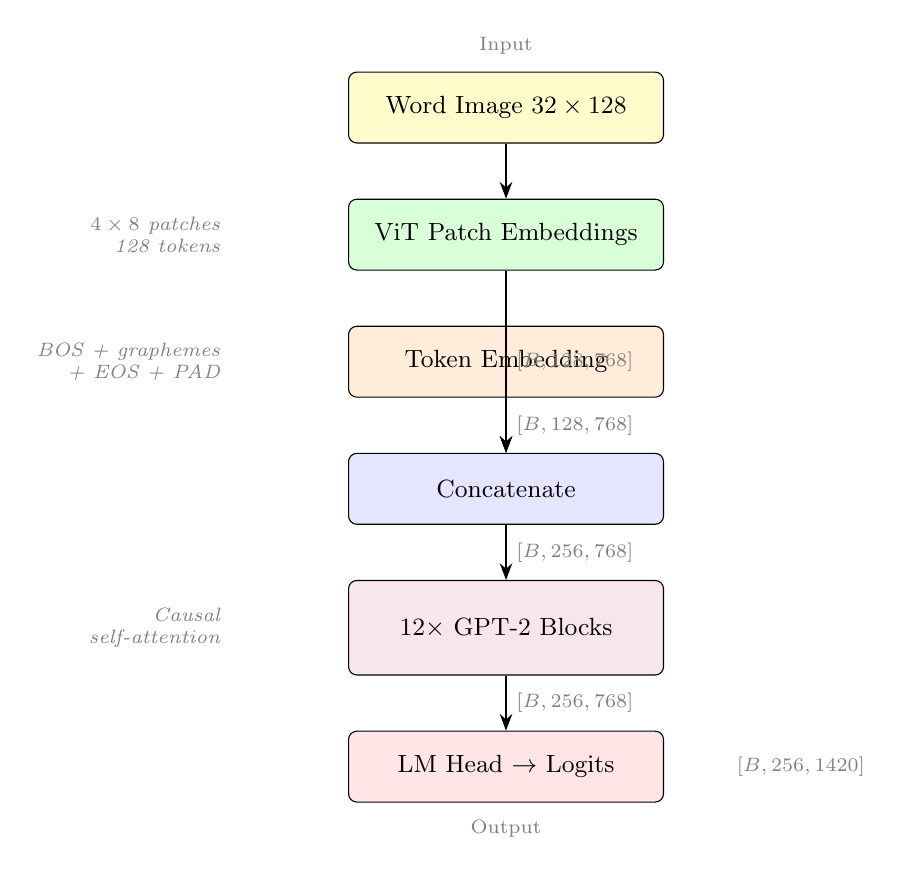
\begin{tikzpicture}[
  block/.style={rectangle, draw, rounded corners=3pt, minimum height=0.9cm, minimum width=4cm, font=\small},
  arrow/.style={-{Stealth[length=6pt]}, thick},
  label/.style={font=\scriptsize\itshape, text=gray},
]
% Nodes
\node[block, fill=yellow!20] (img) {Word Image $32 \times 128$};
\node[block, fill=green!15, below=0.7cm of img] (vit) {ViT Patch Embeddings};
\node[block, fill=orange!15, below=0.7cm of vit] (tok) {Token Embedding};
\node[block, fill=blue!10, below=0.7cm of tok] (cat) {Concatenate};
\node[block, fill=purple!10, below=0.7cm of cat, minimum height=1.2cm] (gpt) {12$\times$ GPT-2 Blocks};
\node[block, fill=red!10, below=0.7cm of gpt] (lm) {LM Head $\to$ Logits};

% Arrows
\draw[arrow] (img) -- (vit);
\draw[arrow] (vit) -- node[right, label] {$[B, 128, 768]$} (cat);
\draw[arrow] (tok) -- node[right, label] {$[B, 128, 768]$} (cat);
\draw[arrow] (cat) -- node[right, label] {$[B, 256, 768]$} (gpt);
\draw[arrow] (gpt) -- node[right, label] {$[B, 256, 768]$} (lm);

% Side labels
\node[left=1.5cm of vit, label, align=right] {$4 \times 8$ patches\\128 tokens};
\node[left=1.5cm of tok, label, align=right] {BOS + graphemes\\+ EOS + PAD};
\node[left=1.5cm of gpt, label, align=right] {Causal\\self-attention};
\node[right=0.8cm of lm, label, align=left] {$[B, 256, 1420]$};

% Input annotation
\node[above=0.1cm of img, font=\scriptsize, gray] {Input};
\node[below=0.1cm of lm, font=\scriptsize, gray] {Output};
\end{tikzpicture}
\caption{Base DTrOCR architecture (without context). The 32$\times$128 word image is divided into 128 patch tokens, concatenated with target grapheme tokens, and processed by 12 GPT-2 blocks with causal attention.}
\label{fig:base-arch}
\end{figure}


\section{Context-Aware Sequence Design}
\label{sec:context-sequence}

The extension prepends context tokens (from the previous word) \emph{before} the image patches, creating the contextual sequence:
\begin{equation}
  \mathbf{S}_{\mathrm{ctx}} = [\underbrace{c_1, \ldots, c_K, \text{SEP}, \text{PAD}, \ldots}_{\text{$C$ context tokens (padded)}},\; \underbrace{\text{IMG}_1, \ldots, \text{IMG}_{128}}_{\text{128 patches}},\; \underbrace{\text{BOS}, t_1, \ldots, t_N, \text{EOS}, \text{PAD}, \ldots}_{\text{128 target tokens}}]
  \label{eq:context-sequence}
\end{equation}
Total: $C + 128 + 128$ positions (where $C = 20$ by default).

\paragraph{Why prepend before image?} Under causal attention, each position can only attend to positions at or before it:
\begin{itemize}[leftmargin=2em]
  \item \textbf{Context tokens} (positions 0 to $C{-}1$): attend only to other context tokens---they serve as a ``prefix prompt.''
  \item \textbf{Image patches} (positions $C$ to $C{+}127$): attend to context tokens \emph{and} other image patches---the visual representation is \emph{conditioned on context}.
  \item \textbf{Target tokens} (positions $C{+}128$ onwards): attend to everything---context, image, and previously generated tokens.
\end{itemize}

\begin{figure}[t]
\centering
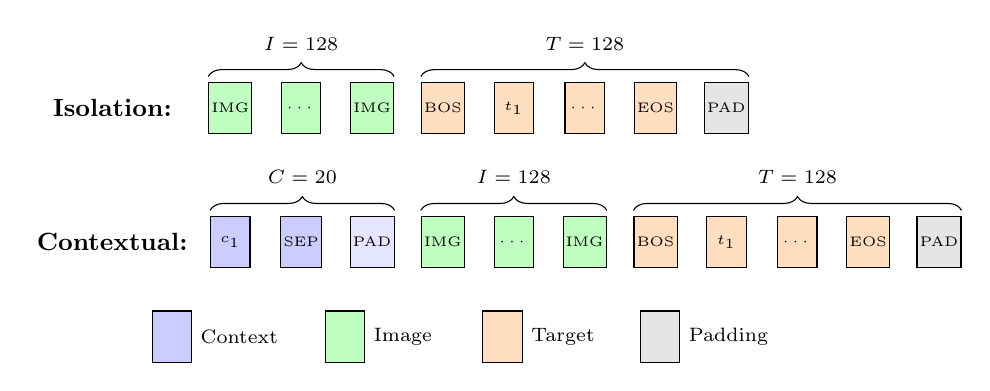
\begin{tikzpicture}[
  box/.style={minimum width=0.5cm, minimum height=0.65cm, draw, font=\tiny, inner sep=1pt},
  brace/.style={decorate, decoration={brace, amplitude=5pt, raise=2pt}},
  lbl/.style={font=\scriptsize, midway, above=8pt},
]
% --- Isolation Path ---
\node[font=\small\bfseries] at (-0.5, 2.2) {Isolation:};
\foreach \i/\c/\t in {0/green!25/IMG, 1/green!25/$\cdots$, 2/green!25/IMG, 3/orange!25/BOS, 4/orange!25/$t_1$, 5/orange!25/$\cdots$, 6/orange!25/EOS, 7/gray!20/PAD}{
  \node[box, fill=\c] (iso\i) at (\i*0.9+1, 2.2) {\t};
}
\draw[brace] (iso0.north west) -- node[lbl] {$I=128$} (iso2.north east);
\draw[brace] (iso3.north west) -- node[lbl] {$T=128$} (iso7.north east);

% --- Contextual Path ---
\node[font=\small\bfseries] at (-0.5, 0.5) {Contextual:};
\foreach \i/\c/\t in {0/blue!20/$c_1$, 1/blue!20/SEP, 2/blue!10/PAD, 3/green!25/IMG, 4/green!25/$\cdots$, 5/green!25/IMG, 6/orange!25/BOS, 7/orange!25/$t_1$, 8/orange!25/$\cdots$, 9/orange!25/EOS, 10/gray!20/PAD}{
  \node[box, fill=\c] (ctx\i) at (\i*0.9+1, 0.5) {\t};
}
\draw[brace] (ctx0.north west) -- node[lbl] {$C=20$} (ctx2.north east);
\draw[brace] (ctx3.north west) -- node[lbl] {$I=128$} (ctx5.north east);
\draw[brace] (ctx6.north west) -- node[lbl] {$T=128$} (ctx10.north east);

% Legend
\node[box, fill=blue!20, anchor=west] at (0, -0.7) {~};
\node[font=\scriptsize, anchor=west] at (0.5, -0.7) {Context};
\node[box, fill=green!25, anchor=west] at (2.2, -0.7) {~};
\node[font=\scriptsize, anchor=west] at (2.7, -0.7) {Image};
\node[box, fill=orange!25, anchor=west] at (4.2, -0.7) {~};
\node[font=\scriptsize, anchor=west] at (4.7, -0.7) {Target};
\node[box, fill=gray!20, anchor=west] at (6.2, -0.7) {~};
\node[font=\scriptsize, anchor=west] at (6.7, -0.7) {Padding};
\end{tikzpicture}
\caption{Sequence structure comparison between isolation mode (top) and contextual mode (bottom). Context tokens ($C{=}20$) are prepended before image patches. Total contextual sequence: $20 + 128 + 128 = 276$ positions.}
\label{fig:sequence-comparison}
\end{figure}


\section{Embedding Reordering Mechanism}
\label{sec:embedding-reorder}

A key design challenge is that the \textbf{processor} outputs tokens in the order $[\text{context}, \text{target}]$ (since it concatenates token IDs), but the \textbf{model} needs them in the order $[\text{context}, \text{IMAGE}, \text{target}]$ (since image patches must be between context and target for correct causal attention). The model's \texttt{DTrOCRModel.forward()} performs this reordering:

\begin{enumerate}[leftmargin=2em]
  \item Compute \texttt{token\_embeddings} $= \mathrm{Embedding}(\texttt{input\_ids})$ --- shape $[B, C{+}T, 768]$
  \item Split: \texttt{context\_emb} $= \texttt{token\_emb}[:, :C, :]$ and \texttt{target\_emb} $= \texttt{token\_emb}[:, C:, :]$
  \item Compute \texttt{patch\_emb} $= \mathrm{ViTPatchEmbeddings}(\texttt{pixel\_values})$ --- shape $[B, 128, 768]$
  \item Concatenate: $[\texttt{context\_emb},\; \texttt{patch\_emb},\; \texttt{target\_emb}]$ --- shape $[B, C{+}128{+}T, 768]$
  \item Add positional embeddings covering the full reordered sequence
\end{enumerate}

\begin{figure}[t]
\centering
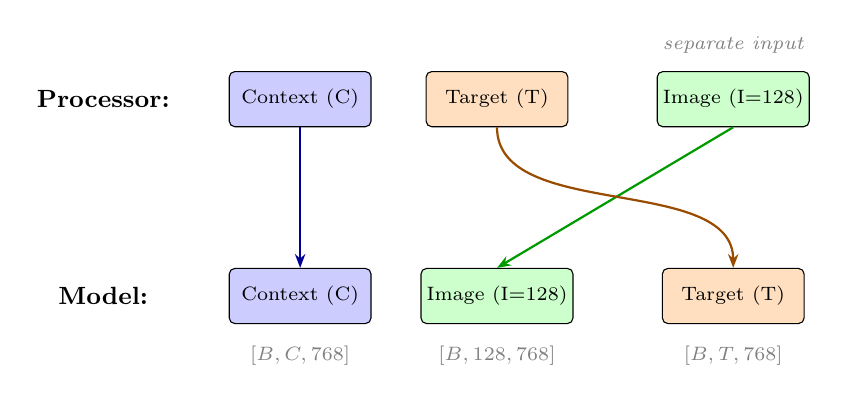
\begin{tikzpicture}[
  box/.style={minimum width=1.8cm, minimum height=0.7cm, draw, rounded corners=2pt, font=\scriptsize, inner sep=2pt},
  arrow/.style={-{Stealth[length=5pt]}, thick},
]
% Top row: Processor output
\node[font=\small\bfseries] at (-2.5, 3) {Processor:};
\node[box, fill=blue!20] (p1) at (0, 3) {Context (C)};
\node[box, fill=orange!25] (p2) at (2.5, 3) {Target (T)};

% Middle: Image
\node[box, fill=green!20] (img) at (5.5, 3) {Image (I=128)};
\node[font=\scriptsize\itshape, gray, above=0.1cm of img] {separate input};

% Bottom row: Model internal
\node[font=\small\bfseries] at (-2.5, 0.5) {Model:};
\node[box, fill=blue!20] (m1) at (0, 0.5) {Context (C)};
\node[box, fill=green!20] (m2) at (2.5, 0.5) {Image (I=128)};
\node[box, fill=orange!25] (m3) at (5.5, 0.5) {Target (T)};

% Arrows
\draw[arrow, blue!60!black] (p1.south) -- (m1.north);
\draw[arrow, green!60!black] (img.south) -- (m2.north);
\draw[arrow, orange!60!black] (p2.south) .. controls +(0,-1.2) and +(0,1.2) .. (m3.north);

% Dimension annotations
\node[font=\scriptsize, gray, below=0.15cm of m1] {$[B, C, 768]$};
\node[font=\scriptsize, gray, below=0.15cm of m2] {$[B, 128, 768]$};
\node[font=\scriptsize, gray, below=0.15cm of m3] {$[B, T, 768]$};
\end{tikzpicture}
\caption{Embedding reordering: the processor outputs \texttt{[context, target]} token IDs, while the model reorders embeddings to \texttt{[context, IMAGE, target]} before passing through GPT-2 blocks.}
\label{fig:embedding-reorder}
\end{figure}


\section{Causal Attention Pattern}
\label{sec:attention-pattern}

\begin{figure}[t]
\centering
\begin{tikzpicture}[scale=0.55]
% Grid
\def\ctx{3}   % context positions
\def\img{4}   % image positions (representative)
\def\tgt{3}   % target positions (representative)
\def\total{10} % ctx+img+tgt

% Background regions
\fill[blue!15] (0,\total-\ctx) rectangle (\ctx,\total);
\fill[green!12] (\ctx,\total-\ctx-\img) rectangle (\ctx+\img,\total);
\fill[green!20] (0,\total-\ctx-\img) rectangle (\ctx,\total-\ctx);
\fill[orange!10] (0,0) rectangle (\total,\total-\ctx-\img);

% Causal mask (lower triangle within each region)
\foreach \r in {0,...,9}{
  \foreach \c in {0,...,\r}{
    \fill[black!50, opacity=0.3] (\c,\total-\r-1) rectangle (\c+1,\total-\r);
  }
}

% Grid lines
\draw[gray!40] (0,0) grid (\total,\total);
\draw[thick] (0,0) rectangle (\total,\total);

% Region boundaries
\draw[blue!60!black, very thick] (\ctx,\total-\ctx) -- (\ctx,\total) -- (0,\total) -- (0,\total-\ctx) -- cycle;
\draw[green!60!black, very thick, dashed] (\ctx,\total-\ctx-\img) -- (\ctx+\img,\total-\ctx-\img) -- (\ctx+\img,\total-\ctx) -- (\ctx,\total-\ctx);
\draw[orange!60!black, very thick, dashed] (0,0) -- (\total,0) -- (\total,\total-\ctx-\img) -- (0,\total-\ctx-\img);

% Labels on axes
\node[font=\footnotesize\bfseries, rotate=90] at (-0.8, \total-\ctx/2) {Ctx};
\node[font=\footnotesize\bfseries, rotate=90] at (-0.8, \total-\ctx-\img/2) {Img};
\node[font=\footnotesize\bfseries, rotate=90] at (-0.8, (\total-\ctx-\img)/2) {Tgt};

\node[font=\footnotesize\bfseries] at (\ctx/2, \total+0.5) {Ctx};
\node[font=\footnotesize\bfseries] at (\ctx+\img/2, \total+0.5) {Img};
\node[font=\footnotesize\bfseries] at (\ctx+\img+\tgt/2, \total+0.5) {Tgt};

% Axis labels
\node[font=\small, above=0.8cm of current bounding box.north] {Key Positions};
\node[font=\small, rotate=90, left=1.5cm of current bounding box.west] {Query Positions};

% Annotations
\draw[{Stealth}-,thick] (\total+0.5, \total-\ctx-2) -- ++(1.5,0.5) node[right, font=\scriptsize, align=left] {Image attends\\to context +\\image};
\draw[{Stealth}-,thick] (\total+0.5, 1) -- ++(1.5,-0.5) node[right, font=\scriptsize, align=left] {Target attends\\to everything};
\end{tikzpicture}
\caption{Causal attention pattern in context mode. Shaded cells indicate attended positions. Context tokens attend only to themselves; image patches attend to context and earlier image patches; target tokens attend to the full prefix (context + image + prior targets).}
\label{fig:attention-pattern}
\end{figure}


\section{Fixed-Length Context Padding}
\label{sec:fixed-padding}

A critical implementation requirement is that all samples in a batch must have identical tensor shapes for \texttt{torch.stack()} in the DataLoader. Since different words have different numbers of context graphemes, na\"ive tokenization produces variable-length tensors---causing a runtime crash.

\paragraph{Solution.} Pad all context tokens to a fixed \texttt{max\_context\_length} $= 20$:
\begin{enumerate}[leftmargin=2em]
  \item Tokenize the previous word text $\to$ variable-length token sequence $(c_1, \ldots, c_k)$
  \item Truncate to at most $\texttt{max\_context\_length} - 1 = 19$ tokens
  \item Append SEP token (reusing \texttt{eos\_token\_id})
  \item Pad with \texttt{pad\_token\_id} to exactly 20 tokens
  \item Set attention mask: 1 for real tokens + SEP, 0 for padding
\end{enumerate}

Result: \texttt{context\_length} $= 20$ for \emph{every} sample, enabling uniform batching.

\section{Position Embedding Budget}
\label{sec:position-budget}

With context, the total sequence length becomes $C + I + T = 20 + 128 + 128 = 276$, exceeding the original \texttt{max\_position\_embeddings} $= 256$. The solution is to increase \texttt{max\_position\_embeddings} to 320, creating a new positional embedding matrix $\mathbf{P} \in \mathbb{R}^{320 \times 768}$. Positions 0--255 can be initialized from the pretrained model; positions 256--319 are randomly initialized and learned during context-aware fine-tuning. This adds approximately 49K parameters ($< 0.06\%$ of the 87M total), a negligible overhead.


% ============================================================================
\chapter{Data Pipeline}
\label{ch:data}
% ============================================================================

\section{JSON Data Format and Context Construction}
\label{sec:json-format}

Context-aware training uses JSON files (one per word image) containing:
\begin{lstlisting}[style=pythonstyle, frame=single, numbers=none]
{"output_path": "path/to/word_image.jpg", "text": "target_text"}
\end{lstlisting}

The \texttt{ContextAwareDataset} constructs previous-word context via a simple shift operation on the DataFrame:
\begin{lstlisting}[style=pythonstyle, frame=single, numbers=none]
df['prev_text'] = df['text'].shift(1).fillna("")
\end{lstlisting}
The first word of each document receives an empty string as context, making it equivalent to isolation mode.


\section{ContextAwareDataset Class}
\label{sec:context-dataset}

Each call to \texttt{\_\_getitem\_\_} produces dual-path data by processing the same image twice:

\begin{table}[h]
\centering
\caption{Dataset output dictionary structure per sample.}
\label{tab:dataset-output}
\begin{tabularx}{\textwidth}{llcX}
\toprule
\textbf{Key} & \textbf{Type} & \textbf{Shape} & \textbf{Description} \\
\midrule
\texttt{pixel\_values} & FloatTensor & $[3, 32, 128]$ & Preprocessed word image (shared) \\
\texttt{input\_ids} & LongTensor & $[C{+}T]$ & Context + target token IDs \\
\texttt{attention\_mask} & LongTensor & $[C{+}T]$ & 1 for real, 0 for padding \\
\texttt{labels} & LongTensor & $[C{+}T]$ & Same as input\_ids (teacher forcing) \\
\texttt{context\_length} & int & scalar & Always $= C = 20$ \\
\midrule
\texttt{input\_ids\_isolated} & LongTensor & $[T]$ & Target-only token IDs \\
\texttt{attention\_mask\_isolated} & LongTensor & $[T]$ & Target-only mask \\
\texttt{labels\_isolated} & LongTensor & $[T]$ & Target-only labels \\
\texttt{context\_length\_isolated} & int & scalar & Always $= 0$ \\
\bottomrule
\end{tabularx}
\end{table}

\section{Processor Context Tokenization Pipeline}
\label{sec:processor-pipeline}

\begin{figure}[t]
\centering
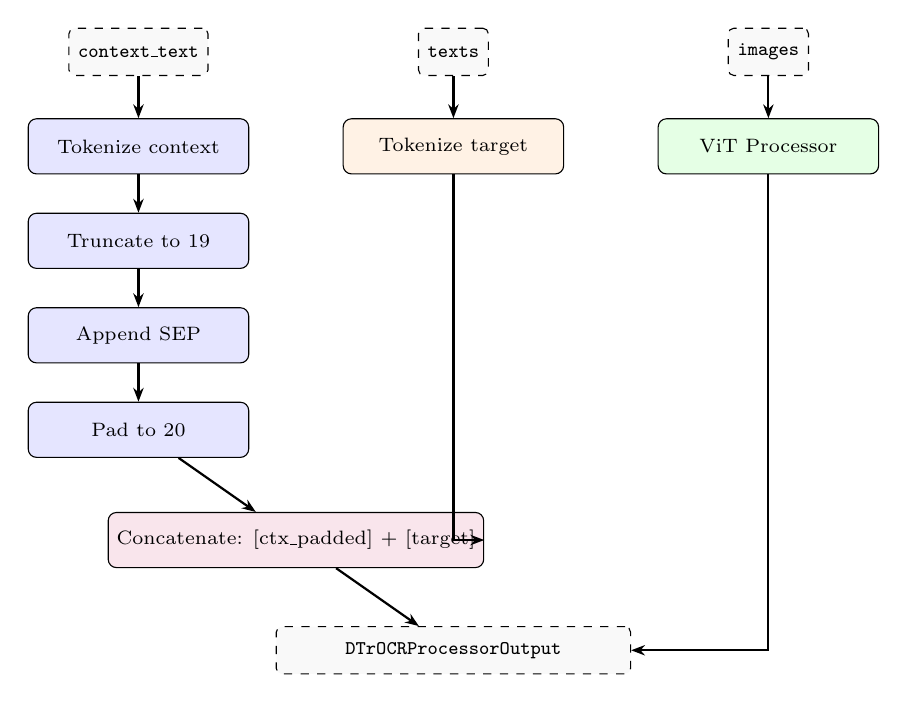
\begin{tikzpicture}[
  proc/.style={rectangle, draw, rounded corners=3pt, minimum height=0.7cm, minimum width=2.8cm, font=\scriptsize, inner sep=3pt},
  data/.style={rectangle, draw, dashed, rounded corners=2pt, minimum height=0.6cm, font=\scriptsize, fill=gray!5},
  arrow/.style={-{Stealth[length=5pt]}, thick},
  decision/.style={diamond, draw, aspect=2.5, font=\scriptsize, inner sep=1pt},
]
% Input
\node[data] (ctx_in) at (0, 4) {\texttt{context\_text}};
\node[data] (txt_in) at (4, 4) {\texttt{texts}};
\node[data] (img_in) at (8, 4) {\texttt{images}};

% Context branch
\node[proc, fill=blue!10] (tok_ctx) at (0, 2.8) {Tokenize context};
\node[proc, fill=blue!10] (trunc) at (0, 1.6) {Truncate to 19};
\node[proc, fill=blue!10] (sep) at (0, 0.4) {Append SEP};
\node[proc, fill=blue!10] (pad) at (0, -0.8) {Pad to 20};

% Target branch
\node[proc, fill=orange!10] (tok_tgt) at (4, 2.8) {Tokenize target};

% Image branch
\node[proc, fill=green!10] (vit) at (8, 2.8) {ViT Processor};

% Merge
\node[proc, fill=purple!10, minimum width=4cm] (merge) at (2, -2.2) {Concatenate: [ctx\_padded] + [target]};

% Output
\node[data, minimum width=4.5cm] (out) at (4, -3.6) {\texttt{DTrOCRProcessorOutput}};

% Arrows
\draw[arrow] (ctx_in) -- (tok_ctx);
\draw[arrow] (tok_ctx) -- (trunc);
\draw[arrow] (trunc) -- (sep);
\draw[arrow] (sep) -- (pad);
\draw[arrow] (pad) -- (merge);
\draw[arrow] (txt_in) -- (tok_tgt);
\draw[arrow] (tok_tgt) |- (merge);
\draw[arrow] (img_in) -- (vit);
\draw[arrow] (vit) |- (out);
\draw[arrow] (merge) -- (out);
\end{tikzpicture}
\caption{Processor data flow for context-aware mode. Context text is tokenized, truncated, given a SEP separator, and padded to a fixed length. It is then concatenated with target token IDs. The image is processed independently through the ViT processor.}
\label{fig:processor-flow}
\end{figure}


% ============================================================================
\chapter{Training Phase}
\label{ch:training}
% ============================================================================

\section{Training Loop Overview}
\label{sec:training-overview}

The training script accepts configurable hyperparameters via \texttt{argparse}:

\begin{lstlisting}[style=pythonstyle, frame=single, numbers=none]
python train.py --context --margin_lambda 0.5 --batch_size 32 --epochs 10 --lr 1e-4
\end{lstlisting}

Mode selection: \texttt{--context} enables dual-path training with the \texttt{ContextAwareDataset}; without it, the standard single-path training runs with \texttt{HandwrittenDataset}.

\section{Dual-Path Training Algorithm}
\label{sec:algorithm}

\begin{algorithm}[t]
\caption{Context-Aware Dual-Path Training}
\label{alg:training}
\begin{algorithmic}[1]
\Require Dataset $\mathcal{D}$, model $M_\theta$, margin weight $\lambda$, epochs $E$
\For{epoch $= 1$ \textbf{to} $E$}
  \For{batch $\mathcal{B} \in \mathcal{D}$}
    \State $\mathbf{x} \gets \mathcal{B}.\texttt{pixel\_values}$ \Comment{Shared image input}
    \Statex
    \State \textcolor{blue}{\textbf{// Forward Pass 1: Contextual Path}}
    \State $\hat{\mathbf{y}}_{\mathrm{ctx}} \gets M_\theta(\mathbf{x},\; \mathcal{B}.\texttt{input\_ids},\; \texttt{context\_length}{=}C)$
    \State $\boldsymbol\ell^{\mathrm{ctx}} \gets \textsc{PerSampleLoss}(\hat{\mathbf{y}}_{\mathrm{ctx}},\; \mathcal{B}.\texttt{labels})$ \Comment{Shape: $[B]$}
    \Statex
    \State \textcolor{orange}{\textbf{// Forward Pass 2: Isolation Path}}
    \State $\hat{\mathbf{y}}_{\mathrm{iso}} \gets M_\theta(\mathbf{x},\; \mathcal{B}.\texttt{input\_ids\_iso},\; \texttt{context\_length}{=}0)$
    \State $\boldsymbol\ell^{\mathrm{iso}} \gets \textsc{PerSampleLoss}(\hat{\mathbf{y}}_{\mathrm{iso}},\; \mathcal{B}.\texttt{labels\_iso})$ \Comment{Shape: $[B]$}
    \Statex
    \State \textcolor{red}{\textbf{// Combined Loss with Margin}}
    \State $\mathbf{m} \gets \lambda \cdot \max(\mathbf{0},\; \boldsymbol\ell^{\mathrm{ctx}} - \boldsymbol\ell^{\mathrm{iso}})$ \Comment{Margin term, shape: $[B]$}
    \State $\mathcal{L} \gets \mathrm{mean}(\boldsymbol\ell^{\mathrm{ctx}} + \boldsymbol\ell^{\mathrm{iso}} + \mathbf{m})$ \Comment{Scalar}
    \Statex
    \State $\theta \gets \theta - \eta \cdot \nabla_\theta \mathcal{L}$ \Comment{Gradient descent (with AMP)}
  \EndFor
  \State Evaluate on validation set (dual-path)
  \State Save checkpoint
\EndFor
\end{algorithmic}
\end{algorithm}


\section{Dimension Trace --- Contextual Path}
\label{sec:dim-trace-ctx}

\Cref{tab:dim-trace-ctx} provides a complete tensor shape trace through the contextual forward pass for a concrete example with batch size $B{=}4$, context length $C{=}20$, target length $T{=}128$, image patches $I{=}128$, hidden dim $H{=}768$, vocabulary $V{=}1420$.

\begin{table}[h]
\centering
\caption{Dimension trace through the contextual forward pass.}
\label{tab:dim-trace-ctx}
\small
\begin{tabular}{llll}
\toprule
\textbf{Stage} & \textbf{Tensor} & \textbf{Shape} & \textbf{Notes} \\
\midrule
Input & \texttt{pixel\_values} & $[4, 3, 32, 128]$ & RGB images \\
Input & \texttt{input\_ids} & $[4, 148]$ & $C{+}T = 20{+}128$ \\
Input & \texttt{attention\_mask} & $[4, 148]$ & \\
\midrule
Embed & \texttt{patch\_embeddings} & $[4, 128, 768]$ & ViT patches \\
Embed & \texttt{token\_embeddings} & $[4, 148, 768]$ & All tokens \\
Split & \texttt{context\_embeddings} & $[4, 20, 768]$ & First $C{=}20$ \\
Split & \texttt{target\_embeddings} & $[4, 128, 768]$ & Remaining $T{=}128$ \\
\midrule
Reorder & \texttt{combined\_embeddings} & $[4, 276, 768]$ & $C{+}I{+}T$ \\
PosMask & \texttt{position\_ids} & $[1, 276]$ & 0\ldots275 \\
PosMask & \texttt{combined\_mask} & $[4, 276]$ & Reordered \\
\midrule
GPT-2 & \texttt{hidden\_states} & $[4, 276, 768]$ & After 12 blocks \\
LM Head & \texttt{logits} & $[4, 276, 1420]$ & Vocab scores \\
\midrule
Loss & \texttt{skip\_positions} & $148$ & $C{+}I = 20{+}128$ \\
Loss & \texttt{shift\_logits} & $[4, 127, 1420]$ & \texttt{logits[..., 148:-1, :]} \\
Loss & \texttt{shift\_labels} & $[4, 127]$ & \texttt{labels[..., 21:]} \\
Loss & \texttt{mask} & $[4, 127]$ & \texttt{attn\_mask[..., 21:]} \\
Loss & \texttt{per\_sample\_loss} & $[4]$ & Masked mean \\
\bottomrule
\end{tabular}
\end{table}


\section{Dimension Trace --- Isolation Path}
\label{sec:dim-trace-iso}

For comparison, the isolation path ($C{=}0$):

\begin{table}[h]
\centering
\caption{Dimension trace through the isolation forward pass.}
\label{tab:dim-trace-iso}
\small
\begin{tabular}{llll}
\toprule
\textbf{Stage} & \textbf{Tensor} & \textbf{Shape} & \textbf{Notes} \\
\midrule
Input & \texttt{input\_ids} & $[4, 128]$ & $T{=}128$ (no context) \\
Reorder & \texttt{combined\_embeddings} & $[4, 256, 768]$ & $I{+}T$ \\
LM Head & \texttt{logits} & $[4, 256, 1420]$ & \\
\midrule
Loss & \texttt{skip\_positions} & $128$ & $0{+}128$ \\
Loss & \texttt{shift\_logits} & $[4, 127, 1420]$ & \texttt{logits[..., 128:-1, :]} \\
Loss & \texttt{shift\_labels} & $[4, 127]$ & \texttt{labels[..., 1:]} \\
\bottomrule
\end{tabular}
\end{table}

Note that when $C{=}0$: \texttt{labels[..., 0+1:] = labels[..., 1:]}---identical to the original code, ensuring backward compatibility.


\section{Validation and Checkpointing}
\label{sec:validation}

The \texttt{evaluate\_context\_model()} function mirrors the training loop but without gradient computation. It reports:
\begin{itemize}[leftmargin=2em]
  \item Combined loss: $\mathcal{L}_{\mathrm{ctx}} + \mathcal{L}_{\mathrm{iso}}$
  \item Individual losses: $\mathcal{L}_{\mathrm{ctx}}$ and $\mathcal{L}_{\mathrm{iso}}$ separately
  \item Average accuracy: $(\mathrm{Acc}_{\mathrm{ctx}} + \mathrm{Acc}_{\mathrm{iso}}) / 2$
\end{itemize}

Checkpoints are saved with the naming convention \texttt{checkpoint\_context\_epoch\_\{N\}.pt} for context mode and \texttt{checkpoint\_epoch\_\{N\}.pt} for standard mode, with the corrected 9-argument signature matching \texttt{save\_checkpoint()} in \texttt{utils.py}.


% ============================================================================
\chapter{Inference with Context}
\label{ch:inference}
% ============================================================================

\section{Sequential Context Propagation}
\label{sec:inference-strategy}

At inference time, context comes from the \emph{previously-recognized} word in the document. The inference proceeds sequentially across words within each line:

\begin{figure}[h]
\centering
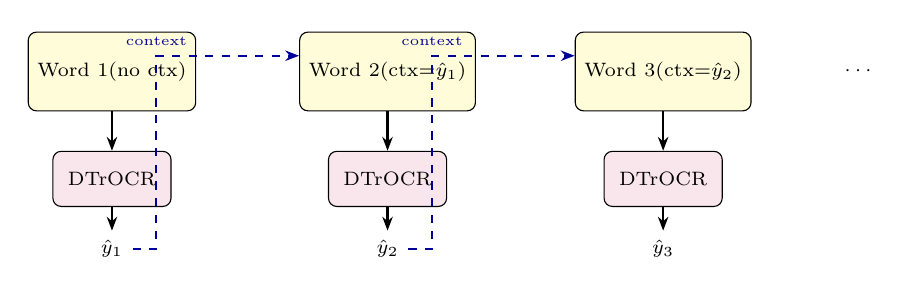
\begin{tikzpicture}[
  word/.style={rectangle, draw, rounded corners=3pt, minimum height=1cm, minimum width=1.8cm, font=\scriptsize, fill=yellow!15},
  model/.style={rectangle, draw, rounded corners=3pt, minimum height=0.7cm, minimum width=1.5cm, font=\scriptsize, fill=purple!10},
  ctxarrow/.style={-{Stealth[length=5pt]}, thick, blue!60!black, dashed},
  arrow/.style={-{Stealth[length=5pt]}, thick},
]
% Words
\node[word] (w1) at (0,0) {Word 1\\(no ctx)};
\node[model, below=0.5cm of w1] (m1) {DTrOCR};
\node[font=\scriptsize, below=0.3cm of m1] (t1) {$\hat{y}_1$};

\node[word] (w2) at (3.5,0) {Word 2\\(ctx=$\hat{y}_1$)};
\node[model, below=0.5cm of w2] (m2) {DTrOCR};
\node[font=\scriptsize, below=0.3cm of m2] (t2) {$\hat{y}_2$};

\node[word] (w3) at (7,0) {Word 3\\(ctx=$\hat{y}_2$)};
\node[model, below=0.5cm of w3] (m3) {DTrOCR};
\node[font=\scriptsize, below=0.3cm of m3] (t3) {$\hat{y}_3$};

\node[font=\scriptsize] at (9.5, 0) {$\cdots$};

% Vertical arrows
\draw[arrow] (w1) -- (m1);
\draw[arrow] (m1) -- (t1);
\draw[arrow] (w2) -- (m2);
\draw[arrow] (m2) -- (t2);
\draw[arrow] (w3) -- (m3);
\draw[arrow] (m3) -- (t3);

% Context flow
\draw[ctxarrow] (t1.east) -- ++(0.3,0) |- ([yshift=0.2cm]w2.west) node[midway, above, font=\tiny, blue!60!black] {context};
\draw[ctxarrow] (t2.east) -- ++(0.3,0) |- ([yshift=0.2cm]w3.west) node[midway, above, font=\tiny, blue!60!black] {context};
\end{tikzpicture}
\caption{Inference pipeline with sequential context propagation. The recognized text of word $i$ becomes the context for recognizing word $i{+}1$. The first word has no context.}
\label{fig:inference-pipeline}
\end{figure}

\section{Current State and Required Modifications}
\label{sec:inference-current}

The current \texttt{generate()} method (model.py:271--340) does \emph{not} pass \texttt{context\_length} during generation---it defaults to 0, meaning inference currently operates in isolation mode only.

To enable context-aware inference, the following modifications are needed:
\begin{enumerate}[leftmargin=2em]
  \item \textbf{Accept context text}: The \texttt{generate()} method should accept an optional \texttt{context\_text} parameter.
  \item \textbf{Process context}: Use the processor with \texttt{context\_text} to create the contextual input sequence.
  \item \textbf{Pass context\_length}: Forward \texttt{context\_length} to the model during the prefill step.
  \item \textbf{KV cache handling}: Context tokens are only processed in the first forward pass (prefill); subsequent autoregressive steps use the KV cache and need no special handling.
  \item \textbf{Orchestration}: The inference script (\texttt{extract\_single\_page.py}) must maintain state---the recognized text of each word---to provide as context for the next word.
\end{enumerate}

\paragraph{Error propagation risk.} If word $i$ is misrecognized, the incorrect text becomes context for word $i{+}1$, potentially causing cascading errors. Mitigation strategies include confidence thresholding (only use context when the model is confident in the previous recognition) and beam search across word boundaries.


% ============================================================================
\chapter{Codebase Changes}
\label{ch:codebase}
% ============================================================================

This chapter provides side-by-side comparisons of all modified files, with original code in \textcolor{red!60!black}{red-bordered} boxes and new extension code in \textcolor{green!60!black}{green-bordered} boxes.

\section{Summary of All Changes}
\label{sec:change-summary}

\begin{table}[h]
\centering
\caption{Summary of all file modifications.}
\label{tab:change-summary}
\begin{tabular}{llccl}
\toprule
\textbf{File} & \textbf{Lines $+/-$} & \textbf{Original} & \textbf{Current} & \textbf{Nature of Change} \\
\midrule
\texttt{config.py} & $+2$ / $-0$ & 48 lines & 50 lines & Added \texttt{max\_context\_length} \\
\texttt{data.py} & $+2$ / $-0$ & 28 lines & 30 lines & Added output fields \\
\texttt{dataset.py} & $+106$ / $-0$ & 58 lines & 164 lines & New \texttt{ContextAwareDataset} \\
\texttt{processor.py} & $+93$ / $-6$ & 58 lines & 151 lines & Context tokenization pipeline \\
\texttt{model.py} & $+82$ / $-28$ & 556 lines & 642 lines & Embedding reorder, loss fix \\
\texttt{train.py} & $+203$ / $-49$ & 82 lines & 252 lines & Dual-path training overhaul \\
\bottomrule
\end{tabular}
\end{table}


\section{\texttt{config.py} --- Added \texttt{max\_context\_length}}
\label{sec:code-config}

\begin{minipage}[t]{0.48\textwidth}
\begin{originalcode}[config.py:22 (parameter list)]
bn_vocab_file: str = '...',
):
\end{originalcode}
\end{minipage}
\hfill
\begin{minipage}[t]{0.48\textwidth}
\begin{newcode}[config.py:22--23 (parameter list)]
bn_vocab_file: str = '...',
max_context_length: Optional[int] = 20,
):
\end{newcode}
\end{minipage}

\vspace{0.5em}
\begin{minipage}[t]{0.48\textwidth}
\begin{originalcode}[config.py:\_\_init\_\_ body]
self.bn_vocab_file = bn_vocab_file
# (no max_context_length)
\end{originalcode}
\end{minipage}
\hfill
\begin{minipage}[t]{0.48\textwidth}
\begin{newcode}[config.py:\_\_init\_\_ body, line 34]
self.max_context_length = max_context_length
self.bn_vocab_file = bn_vocab_file
\end{newcode}
\end{minipage}


\section{\texttt{data.py} --- New Output Fields}
\label{sec:code-data}

\begin{minipage}[t]{0.48\textwidth}
\begin{originalcode}[data.py:DTrOCRLMHeadModelOutput]
@dataclass
class DTrOCRLMHeadModelOutput:
    logits: torch.FloatTensor
    loss: Optional[...] = None
    accuracy: Optional[...] = None
    past_key_values: Optional[...] = None
\end{originalcode}
\end{minipage}
\hfill
\begin{minipage}[t]{0.48\textwidth}
\begin{newcode}[data.py:DTrOCRLMHeadModelOutput]
@dataclass
class DTrOCRLMHeadModelOutput:
    logits: torch.FloatTensor
    loss: Optional[...] = None
    accuracy: Optional[...] = None
    past_key_values: Optional[...] = None
    per_sample_loss: Optional[...] = None  # NEW
\end{newcode}
\end{minipage}

\vspace{0.5em}
\begin{minipage}[t]{0.48\textwidth}
\begin{originalcode}[data.py:DTrOCRProcessorOutput]
@dataclass
class DTrOCRProcessorOutput:
    pixel_values: Optional[...] = None
    input_ids: Optional[...] = None
    attention_mask: Optional[...] = None
    labels: Optional[...] = None
\end{originalcode}
\end{minipage}
\hfill
\begin{minipage}[t]{0.48\textwidth}
\begin{newcode}[data.py:DTrOCRProcessorOutput]
@dataclass
class DTrOCRProcessorOutput:
    pixel_values: Optional[...] = None
    input_ids: Optional[...] = None
    attention_mask: Optional[...] = None
    labels: Optional[...] = None
    context_length: Optional[int] = None  # NEW
\end{newcode}
\end{minipage}


\section{\texttt{dataset.py} --- New \texttt{ContextAwareDataset}}
\label{sec:code-dataset}

The original \texttt{HandwrittenDataset} class (lines 11--43) is \textbf{unchanged}. The following is entirely \textbf{new code}:

\begin{newcode}[dataset.py:46--139 --- ContextAwareDataset (NEW)]
class ContextAwareDataset(Dataset):
    """Dataset for context-aware HTR. Each sample includes
    the current word image and previous word's text as context."""

    def __init__(self, images_dir, json_dir, config, data_frame=None):
        super().__init__()
        self.images_dir = images_dir
        self.json_dir = json_dir
        self.config = config
        if data_frame is None:
            self.df = self._build_dataframe_from_json()
        else:
            self.df = data_frame
        self.processor = DTrOCRProcessor(config, add_eos_token=True, add_bos_token=True)

    def _build_dataframe_from_json(self):
        """Build dataframe from JSON files with previous word context."""
        data = []
        json_files = sorted([f for f in os.listdir(self.json_dir)
                            if f.endswith('.json')])
        for json_file in json_files:
            with open(os.path.join(self.json_dir, json_file), 'r') as f:
                json_data = json.load(f)
            data.append({
                'image_id': os.path.basename(json_data['output_path']),
                'text': json_data['text']
            })
        df = pd.DataFrame(data)
        df['prev_text'] = df['text'].shift(1).fillna("")  # Context
        return df

    def __getitem__(self, index):
        row = self.df.iloc[index]
        image = Image.open(os.path.join(self.images_dir,
                          row['image_id'])).convert('RGB')
        text, prev_text = str(row['text']), str(row['prev_text'])

        # Path 1: WITH context
        inputs_ctx = self.processor(images=image, texts=text,
            context_text=prev_text, padding=True, return_labels=True)

        # Path 2: WITHOUT context (isolation)
        inputs_iso = self.processor(images=image, texts=text,
            context_text="", padding=True, return_labels=True)

        return {
            'pixel_values': inputs_ctx.pixel_values[0],
            'input_ids': inputs_ctx.input_ids[0],
            'attention_mask': inputs_ctx.attention_mask[0],
            'labels': inputs_ctx.labels[0],
            'context_length': inputs_ctx.context_length,
            'input_ids_isolated': inputs_iso.input_ids[0],
            'attention_mask_isolated': inputs_iso.attention_mask[0],
            'labels_isolated': inputs_iso.labels[0],
            'context_length_isolated': inputs_iso.context_length,
        }
\end{newcode}

\begin{newcode}[dataset.py:152--163 --- split\_context\_data (NEW)]
def split_context_data(images_dir, json_dir, config,
                       test_size=0.05, random_seed=42):
    """Split context-aware dataset into train and test sets."""
    dataset = ContextAwareDataset(images_dir, json_dir, config)
    df = dataset.df
    train_df, test_df = train_test_split(df, test_size=test_size,
                                         random_state=random_seed)
    train_dataset = ContextAwareDataset(images_dir, json_dir, config,
                       data_frame=train_df.reset_index(drop=True))
    test_dataset = ContextAwareDataset(images_dir, json_dir, config,
                       data_frame=test_df.reset_index(drop=True))
    return train_dataset, test_dataset
\end{newcode}


\section{\texttt{processor.py} --- Context Tokenization Pipeline}
\label{sec:code-processor}

\begin{minipage}[t]{0.48\textwidth}
\begin{originalcode}[processor.py:\_\_init\_\_ and \_\_call\_\_]
class DTrOCRProcessor:
  def __init__(self, config, ...):
    self.vit_processor = AutoImageProcessor
      .from_pretrained(...)
    self.tokeniser = BnGraphemizerProcessor(
      config.bn_vocab_file, ...)

  def __call__(self, images=None,
      texts=None, return_labels=False,
      ...):
    text_inputs = self.tokeniser(
      texts, padding=padding
    ) if texts is not None else None

    image_inputs = self.vit_processor(
      images, ...
    ) if images is not None else None

    return DTrOCRProcessorOutput(
      pixel_values=...,
      input_ids=...,
      attention_mask=...,
      labels=...
    )
\end{originalcode}
\end{minipage}
\hfill
\begin{minipage}[t]{0.48\textwidth}
\begin{newcode}[processor.py:\_\_init\_\_ and \_\_call\_\_ (extended)]
class DTrOCRProcessor:
  def __init__(self, config, ...):
    self.max_context_length = getattr(
      config, 'max_context_length', 20)  # NEW
    self.vit_processor = ...
    self.tokeniser = ...

  def __call__(self, images=None,
      texts=None,
      context_text=None,  # NEW PARAM
      return_labels=False, ...):
    context_length = 0
    text_inputs = self.tokeniser(texts, ...)

    # --- NEW: Context prepending ---
    if context_text is not None \
       and context_text != "" \
       and text_inputs is not None:
      ctx_ids = self.tokeniser(
        context_text, padding=False)
      ctx_ids = ctx_ids[:max_ctx_len - 1]
      ctx_with_sep = ctx_ids + [SEP]
      # Pad to fixed length
      pad_needed = max_ctx_len - len(ctx_with_sep)
      ctx_padded = ctx_with_sep + [PAD]*pad_needed
      ctx_mask = [1]*len(ctx_with_sep) \
               + [0]*pad_needed
      context_length = max_ctx_len  # FIXED
      combined = ctx_padded + target_ids
      text_inputs['input_ids'] = combined
      text_inputs['attention_mask'] = ...

    return DTrOCRProcessorOutput(
      ...,
      context_length=context_length  # NEW
    )
\end{newcode}
\end{minipage}

\section{\texttt{model.py} --- \texttt{DTrOCRModel.forward()} --- Embedding Reordering}
\label{sec:code-model-transformer}

\begin{minipage}[t]{0.48\textwidth}
\begin{originalcode}[model.py:51--89 (forward signature + embeddings)]
def forward(self, pixel_values, input_ids,
    position_ids=None, past_key_values=None,
    attention_mask=None, use_cache=False,
) -> DTrOCRModelOutput:
    # ...
    patch_emb = self.patch_embeddings(
      pixel_values) if past_length == 0 else None
    token_emb = self.token_embedding(input_ids)

    if patch_emb is not None:
      patch_and_token = torch.concat(
        [patch_emb, token_emb], dim=-2)
    else:
      patch_and_token = token_emb

    # ... attention mask ...
    attention_mask = torch.concat([
      torch.ones(..., patch_emb.shape[-2], ...),
      attention_mask
    ], dim=-1)
\end{originalcode}
\end{minipage}
\hfill
\begin{minipage}[t]{0.48\textwidth}
\begin{newcode}[model.py:43--143 (extended forward)]
def forward(self, pixel_values, input_ids,
    position_ids=None, past_key_values=None,
    attention_mask=None, use_cache=False,
    context_length: int = 0,        # NEW
) -> DTrOCRModelOutput:
    # ...
    patch_emb = self.patch_embeddings(...)
    token_emb = self.token_embedding(input_ids)

    # NEW: 3-way reorder
    if patch_emb is not None and context_length > 0:
      ctx_emb = token_emb[:, :context_length, :]
      tgt_emb = token_emb[:, context_length:, :]
      combined = torch.concat([
        ctx_emb, patch_emb, tgt_emb], dim=-2)
    elif patch_emb is not None:
      combined = torch.concat(
        [patch_emb, token_emb], dim=-2)
    else:
      combined = token_emb

    # NEW: 3-way mask reorder
    if context_length > 0 and patch_emb is not None:
      ctx_mask = attn_mask[:, :context_length]
      tgt_mask = attn_mask[:, context_length:]
      patch_mask = torch.ones(..., 128, ...)
      attn_mask = torch.concat(
        [ctx_mask, patch_mask, tgt_mask], dim=-1)
    else:
      # Original behavior
      attn_mask = torch.concat(
        [torch.ones(...), attn_mask], dim=-1)
\end{newcode}
\end{minipage}


\section{\texttt{model.py} --- \texttt{DTrOCRLMHeadModel.forward()} --- Loss Computation}
\label{sec:code-model-lm}

This is the most critical change, fixing Bugs 1 and 2:

\begin{minipage}[t]{0.48\textwidth}
\begin{originalcode}[model.py:148--176 (loss computation)]
def forward(self, pixel_values, input_ids,
    ..., labels=None,
) -> DTrOCRLMHeadModelOutput:
    transformer_output = self.transformer(
      pixel_values=pixel_values,
      input_ids=input_ids, ...)
    logits = self.language_model_head(...)

    loss, accuracy = None, None
    if labels is not None:
      shift_logits = logits[...,
        self.image_embedding_length:-1, :]
      shift_labels = labels[..., 1:]

      loss_fct = CrossEntropyLoss(reduction="none")
      loss = loss_fct(shift_logits.view(-1, ...),
                      shift_labels.view(-1))
      # ...
      if attention_mask is not None:
        mask = attention_mask[..., 1:].reshape(-1)
        loss = (mask * loss).sum() / mask.sum()
        accuracy = (mask * matches).sum() / mask.sum()
      else:
        loss = loss.mean()

    return DTrOCRLMHeadModelOutput(
      loss=loss, logits=logits,
      accuracy=accuracy, ...)
\end{originalcode}
\end{minipage}
\hfill
\begin{minipage}[t]{0.48\textwidth}
\begin{newcode}[model.py:184--268 (fixed loss + per-sample)]
def forward(self, pixel_values, input_ids,
    ..., labels=None,
    context_length: int = 0,           # NEW
    return_per_sample_loss: bool=False, # NEW
) -> DTrOCRLMHeadModelOutput:
    transformer_output = self.transformer(
      ..., context_length=context_length) # NEW
    logits = self.language_model_head(...)

    loss, accuracy, per_sample_loss = None,None,None
    if labels is not None:
      # FIX: skip context + image positions
      skip = context_length + self.image_emb_len
      shift_logits = logits[..., skip:-1, :]
      # FIX: skip context tokens in labels
      shift_labels = labels[...,
        context_length + 1:]

      loss_fct = CrossEntropyLoss(reduction="none")
      loss_per_token = loss_fct(...)

      # NEW: per-sample computation
      loss_2d = loss_per_token.view(B, seq_len)
      if attention_mask is not None:
        # FIX: skip context in mask
        mask = attention_mask[...,
          context_length + 1:].reshape(B, seq_len)
        per_sample_loss = (mask * loss_2d).sum(1) \
                        / mask.sum(1)
        loss = per_sample_loss.mean()

    return DTrOCRLMHeadModelOutput(
      ..., per_sample_loss=per_sample_loss
      if return_per_sample_loss else None)  # NEW
\end{newcode}
\end{minipage}

\paragraph{Key changes marked:}
\begin{itemize}[leftmargin=2em]
  \item \textbf{Bug 1 Fix (line 227):} \texttt{labels[..., 1:]} $\to$ \texttt{labels[..., context\_length + 1:]}
  \item \textbf{Bug 2 Fix (line 248):} \texttt{attention\_mask[..., 1:]} $\to$ \texttt{attention\_mask[..., context\_length + 1:]}
  \item \textbf{New:} \texttt{context\_length} and \texttt{return\_per\_sample\_loss} parameters
  \item \textbf{New:} Per-sample loss computation with 2D reshape
\end{itemize}

\section{\texttt{train.py} --- Complete Overhaul}
\label{sec:code-train}

\begin{minipage}[t]{0.48\textwidth}
\begin{originalcode}[train.py (original --- 82 lines, no context)]
import tqdm
from utils import ... , evaluate_model, ...
from dataset import split_data
# No argparse
# Hardcoded paths
images_dir = "../sample_train/images"
labels_file = "../sample_train/labels/label.csv"
config = DTrOCRConfig()
train_ds, val_ds = split_data(...)
# Hardcoded hyperparameters
train_dl = DataLoader(train_ds, batch_size=32, ...)
model = DTrOCRLMHeadModel(config)
model = torch.compile(model)  # Required
optimizer = torch.optim.Adam(..., lr=1e-4)
EPOCHS = 10

for epoch in range(EPOCHS):
  for inputs in tqdm.tqdm(train_dl, ...):
    optimizer.zero_grad()
    inputs = send_inputs_to_device(inputs, ...)
    with torch.autocast(...):
      outputs = model(**inputs)
    scaler.scale(outputs.loss).backward()
    scaler.step(optimizer)
    scaler.update()
    epoch_losses.append(outputs.loss.item())

  val_loss, val_acc = evaluate_model(...)
  print(f"Epoch {epoch+1} ...")
  # No checkpoint saving
  # No final model saving
\end{originalcode}
\end{minipage}
\hfill
\begin{minipage}[t]{0.48\textwidth}
\begin{newcode}[train.py (new --- 252 lines, dual-path)]
import tqdm, argparse           # NEW
from utils import ..., save_checkpoint, save_final_model
from dataset import split_data, split_context_data

# NEW: argparse with 7 parameters
parser = argparse.ArgumentParser(...)
parser.add_argument('--context', ...)
parser.add_argument('--margin_lambda', default=0.5)
parser.add_argument('--batch_size', '--epochs', '--lr')
args = parser.parse_args()

# NEW: mode selection
if args.context:
  train_ds, val_ds = split_context_data(...)
else:
  train_ds, val_ds = split_data(...)

# Bug 3 fix: function BEFORE loop
def evaluate_context_model(model, dl, device):
  """Dual-path validation."""  # 40 lines
  ...

for epoch in range(EPOCHS):
  for inputs in tqdm.tqdm(train_dl, ...):
    if args.context:
      # NEW: dual-path forward
      out_ctx = model(..., context_length=C,
                      return_per_sample_loss=True)
      out_iso = model(..., context_length=0,
                      return_per_sample_loss=True)
      # Bug 4 fix: margin loss
      base = per_sample_ctx + per_sample_iso
      margin = lambda * clamp(ctx - iso, min=0)
      loss = (base + margin).mean()
    else:
      # Standard (unchanged)
      outputs = model(**inputs)
      loss = outputs.loss

  # Bug 6 fix: correct save_checkpoint args
  save_checkpoint(model, optimizer, epoch+1,
    train_loss, val_loss, train_acc, val_acc,
    './', f'checkpoint_...epoch_{epoch+1}.pt')
save_final_model(model, 'final_...model.pth')
\end{newcode}
\end{minipage}


% ============================================================================
\chapter{Bug Discovery and Resolution}
\label{ch:bugs}
% ============================================================================

The context-aware extension initially contained 6 bugs that prevented training from completing a single epoch. These were discovered through systematic code auditing and resolved in commits \texttt{d162227} and \texttt{3b72a7d}.

\section{Bug Summary}
\label{sec:bug-summary}

\begin{table}[h]
\centering
\caption{All 6 bugs discovered, in crash order. Red rows crash; yellow is a silent logic error.}
\label{tab:bug-summary}
\small
\begin{tabularx}{\textwidth}{clllcX}
\toprule
\textbf{\#} & \textbf{File:Line} & \textbf{Type} & \textbf{Crash?} & \textbf{Order} & \textbf{Fix Applied} \\
\midrule
\rowcolor{red!8}
5 & \texttt{processor.py:79} & Variable-length context & Yes & 1st & Fixed-length padding to $C{=}20$ \\
\rowcolor{red!8}
1 & \texttt{model.py:227} & Label dim mismatch & Yes & 2nd & \texttt{labels[..., ctx\_len+1:]} \\
\rowcolor{red!8}
2 & \texttt{model.py:248} & Mask reshape mismatch & Yes & 3rd & \texttt{attn\_mask[..., ctx\_len+1:]} \\
\rowcolor{red!8}
3 & \texttt{train.py:176} & Func before definition & Yes & 4th & Moved function above loop \\
\rowcolor{red!8}
6 & \texttt{train.py:194} & Wrong save\_checkpoint args & Yes & 5th & Fixed to 9 arguments \\
\rowcolor{yellow!15}
4 & \texttt{train.py:124} & Wrong loss formula & No & Always & Replaced with margin term \\
\bottomrule
\end{tabularx}
\end{table}

\section{Bug 1 --- Label Dimension Mismatch}
\label{sec:bug1}

\paragraph{Location:} \texttt{model.py}, line 225 (original), \texttt{DTrOCRLMHeadModel.forward()}

\paragraph{Problem.} The original code shifts labels with \texttt{labels[..., 1:]} producing shape $[B, C{+}T{-}1]$, but \texttt{shift\_logits} (after skipping context + image positions) has shape $[B, T{-}1, V]$. When $C > 0$, $C{+}T{-}1 \neq T{-}1$, causing \texttt{CrossEntropyLoss} to fail with a size mismatch error.

\paragraph{Numerical trace} ($C{=}3$, $T{=}6$, $I{=}128$):
\begin{align*}
  \texttt{shift\_logits} &= \texttt{logits[..., 131:-1, :]} \quad \text{shape: } [B, 5, V] \quad (T{-}1 = 5) \\
  \texttt{shift\_labels (BUG)} &= \texttt{labels[..., 1:]} \quad \text{shape: } [B, 8] \quad (C{+}T{-}1 = 8) \\
  \texttt{shift\_labels (FIX)} &= \texttt{labels[..., 4:]} \quad \text{shape: } [B, 5] \quad (T{-}1 = 5) \; \checkmark
\end{align*}

\paragraph{Backward compatibility.} When $C{=}0$: \texttt{labels[..., 0+1:] = labels[..., 1:]}---identical to original.

\section{Bug 2 --- Attention Mask Reshape Mismatch}
\label{sec:bug2}

\paragraph{Location:} \texttt{model.py}, line 246 (original)

\paragraph{Problem.} The \texttt{attention\_mask} variable in \texttt{DTrOCRLMHeadModel.forward()} is the \emph{original, un-reordered} mask from the caller (shape $[B, C{+}T]$), not the reordered mask inside \texttt{DTrOCRModel.forward()}. Python's parameter passing means rebinding the local variable inside the inner function does not affect the outer reference. The reshape \texttt{.reshape(B, T{-}1)} fails because $C{+}T{-}1 \neq T{-}1$.

\paragraph{Fix.} Same pattern as Bug 1: \texttt{attention\_mask[..., context\_length + 1:]}.

\section{Bug 3 --- Function Called Before Definition}
\label{sec:bug3}

\paragraph{Location:} \texttt{train.py}, line 176 (call) vs.\ line 202 (definition)

\paragraph{Problem.} Python executes module-level code top-to-bottom. The training loop at line 69 begins before the interpreter reaches the \texttt{evaluate\_context\_model} definition at line 202. When the first epoch ends and validation is invoked at line 176, a \texttt{NameError} results.

\paragraph{Fix.} Move the function definition to before the training loop (now at line 63).

\section{Bug 4 --- Wrong Loss Formula}
\label{sec:bug4}

\paragraph{Location:} \texttt{train.py}, lines 124--135 (original)

\paragraph{Problem.} The original code implemented \emph{difficulty weighting} (upweighting hard samples based on isolation loss) instead of the intended \emph{margin penalty} (penalizing samples where context hurts). See \Cref{tab:loss-comparison} for the mathematical comparison.

\paragraph{Fix.} Replace with the margin term:
\begin{lstlisting}[style=pythonstyle, frame=single, numbers=none]
margin_term = args.margin_lambda * torch.clamp(
    per_sample_loss_ctx - per_sample_loss_iso, min=0.0)
weighted_loss = (combined_base_loss + margin_term).mean()
\end{lstlisting}

\section{Bug 5 --- Variable-Length Context Breaking DataLoader}
\label{sec:bug5}

\paragraph{Location:} \texttt{processor.py}, lines 79--125 (original)

\paragraph{Severity:} \textbf{Critical}---crashes immediately when DataLoader forms the first batch.

\paragraph{Problem.} Context was tokenized without padding, producing variable-length \texttt{input\_ids} tensors. When the DataLoader calls \texttt{torch.stack()}, tensors of different lengths cause a \texttt{RuntimeError}.

\paragraph{Additionally:} Even within a batch, \texttt{context\_length} varied per sample. The training loop took only \texttt{inputs['context\_length'][0].item()}---the first sample's value---silently applying the wrong offset for all other samples.

\paragraph{Fix.} Pad all contexts to fixed \texttt{max\_context\_length = 20} with truncation, SEP token, and padding (see \Cref{sec:fixed-padding}).

\section{Bug 6 --- \texttt{save\_checkpoint} Argument Mismatch}
\label{sec:bug6}

\paragraph{Location:} \texttt{train.py}, line 194 (original)

\paragraph{Problem.} The function \texttt{save\_checkpoint()} in \texttt{utils.py} expects 9 positional arguments: \texttt{model, optimizer, epoch, train\_loss, val\_loss, train\_acc, val\_acc, checkpoint\_dir, checkpoint\_name}. The original call passed only 6 arguments, causing a \texttt{TypeError}.

\paragraph{Fix.} Add the missing \texttt{train\_accuracies[-1]}, \texttt{validation\_accuracies[-1]}, and \texttt{'./'} arguments.


% ============================================================================
\chapter{Test Infrastructure}
\label{ch:tests}
% ============================================================================

\section{Test Suite Overview}
\label{sec:test-overview}

The extension includes a comprehensive test suite of 11 files:

\begin{table}[h]
\centering
\caption{Test files in the \texttt{test\_scripts/} directory.}
\label{tab:test-files}
\small
\begin{tabularx}{\textwidth}{lX}
\toprule
\textbf{File} & \textbf{Description} \\
\midrule
\texttt{00\_run\_all\_tests.sh} & Master orchestrator (\texttt{--quick} or \texttt{--full} mode) \\
\texttt{01\_test\_dataset\_loading.py} & Standard and context dataset loading validation \\
\texttt{02\_test\_model\_forward.py} & Forward pass dimensions, dual-path, difficulty weights \\
\texttt{03\_quick\_train\_standard.sh} & Quick standard training run (1 epoch) \\
\texttt{04\_quick\_train\_context.sh} & Quick context training run (1 epoch) \\
\texttt{05\_train\_context\_full.sh} & Full context training \\
\texttt{06\_compare\_context\_vs\_standard.sh} & Side-by-side comparison \\
\texttt{07\_test\_all\_batch\_sizes.sh} & Batch size sweep \\
\texttt{08\_test\_learning\_rates.sh} & Learning rate sweep \\
\texttt{09\_validate\_context\_benefit.py} & Statistical validation that context helps \\
\texttt{10\_diagnostic\_context\_suite.py} & Comprehensive diagnostic: 18 test cases, 1020 lines \\
\bottomrule
\end{tabularx}
\end{table}

\section{Key Diagnostic Tests}
\label{sec:diagnostic-tests}

The comprehensive diagnostic suite (\texttt{10\_diagnostic\_context\_suite.py}) covers:

\begin{enumerate}[leftmargin=2em]
  \item \textbf{Tests 1--2}: Isolation and context forward pass dimension traces
  \item \textbf{Test 3}: Shift alignment sweep across $C \in \{0, 1, 2, \ldots, 25\}$---verifies \texttt{shift\_logits} and \texttt{shift\_labels} match for every context length
  \item \textbf{Test 4}: Label content correctness (the actual token IDs are correct, not just shapes)
  \item \textbf{Test 5}: Attention mask alignment (mask has correct length after context skip)
  \item \textbf{Tests 6--7}: Margin term activation logic and full loss formula numerical verification
  \item \textbf{Test 8}: Full dual-path forward pass simulation
  \item \textbf{Test 9}: Gradient flow verification (gradients are non-zero and finite)
  \item \textbf{Test 10}: Backward compatibility with \texttt{context\_length=0}
  \item \textbf{Tests 11--12}: Edge cases (batch\_size=1, heavy padding at 90\%)
  \item \textbf{Test 13}: Processor fixed-length context padding verification
  \item \textbf{Test 14}: DataLoader stacking simulation (the original Bug 5 crash scenario)
  \item \textbf{Test 15}: \texttt{save\_checkpoint} signature inspection
  \item \textbf{Test 16}: \texttt{evaluate\_context\_model} definition order check
  \item \textbf{Test 17}: Position embedding budget validation ($C + I + T \leq$ \texttt{max\_position\_embeddings})
  \item \textbf{Test 18}: Margin term with actual model outputs (end-to-end)
\end{enumerate}


% ============================================================================
\chapter{Discussion and Future Work}
\label{ch:discussion}
% ============================================================================

\section{Architectural Trade-offs}
\label{sec:tradeoffs}

\paragraph{Shared weights.} Both the contextual and isolation paths share the same transformer weights. This is computationally expensive (2 forward passes per sample) but ensures the model learns a unified representation that works with or without context.

\paragraph{Fixed context length.} Padding all contexts to $C{=}20$ wastes some positions on short context words. Dynamic batching (grouping similar-length contexts) could improve efficiency but adds complexity.

\paragraph{Position embedding extension.} Increasing \texttt{max\_position\_embeddings} from 256 to 320 means positions 256--319 are randomly initialized. When fine-tuning a pretrained model, these new positions start without prior knowledge---early training may be unstable for samples that use the extended range.

\section{Limitations}
\label{sec:limitations}

\begin{enumerate}[leftmargin=2em]
  \item \textbf{Error propagation}: At inference, a misrecognized word provides incorrect context for the next word, potentially causing cascading errors.
  \item \textbf{Single-word context}: The current design uses only the immediately preceding word. A sliding window over multiple previous words could capture richer linguistic context.
  \item \textbf{Inference not yet implemented}: The \texttt{generate()} method does not currently support context-aware decoding. This is a training-only extension.
  \item \textbf{No benchmark results yet}: The context-aware model has not been evaluated on BN-HTRd or Bongabdo benchmarks.
\end{enumerate}







\end{document}
